\section{Prompt designs}
\label{app:prompts}

\begin{figure*}[h]
\begin{center}
    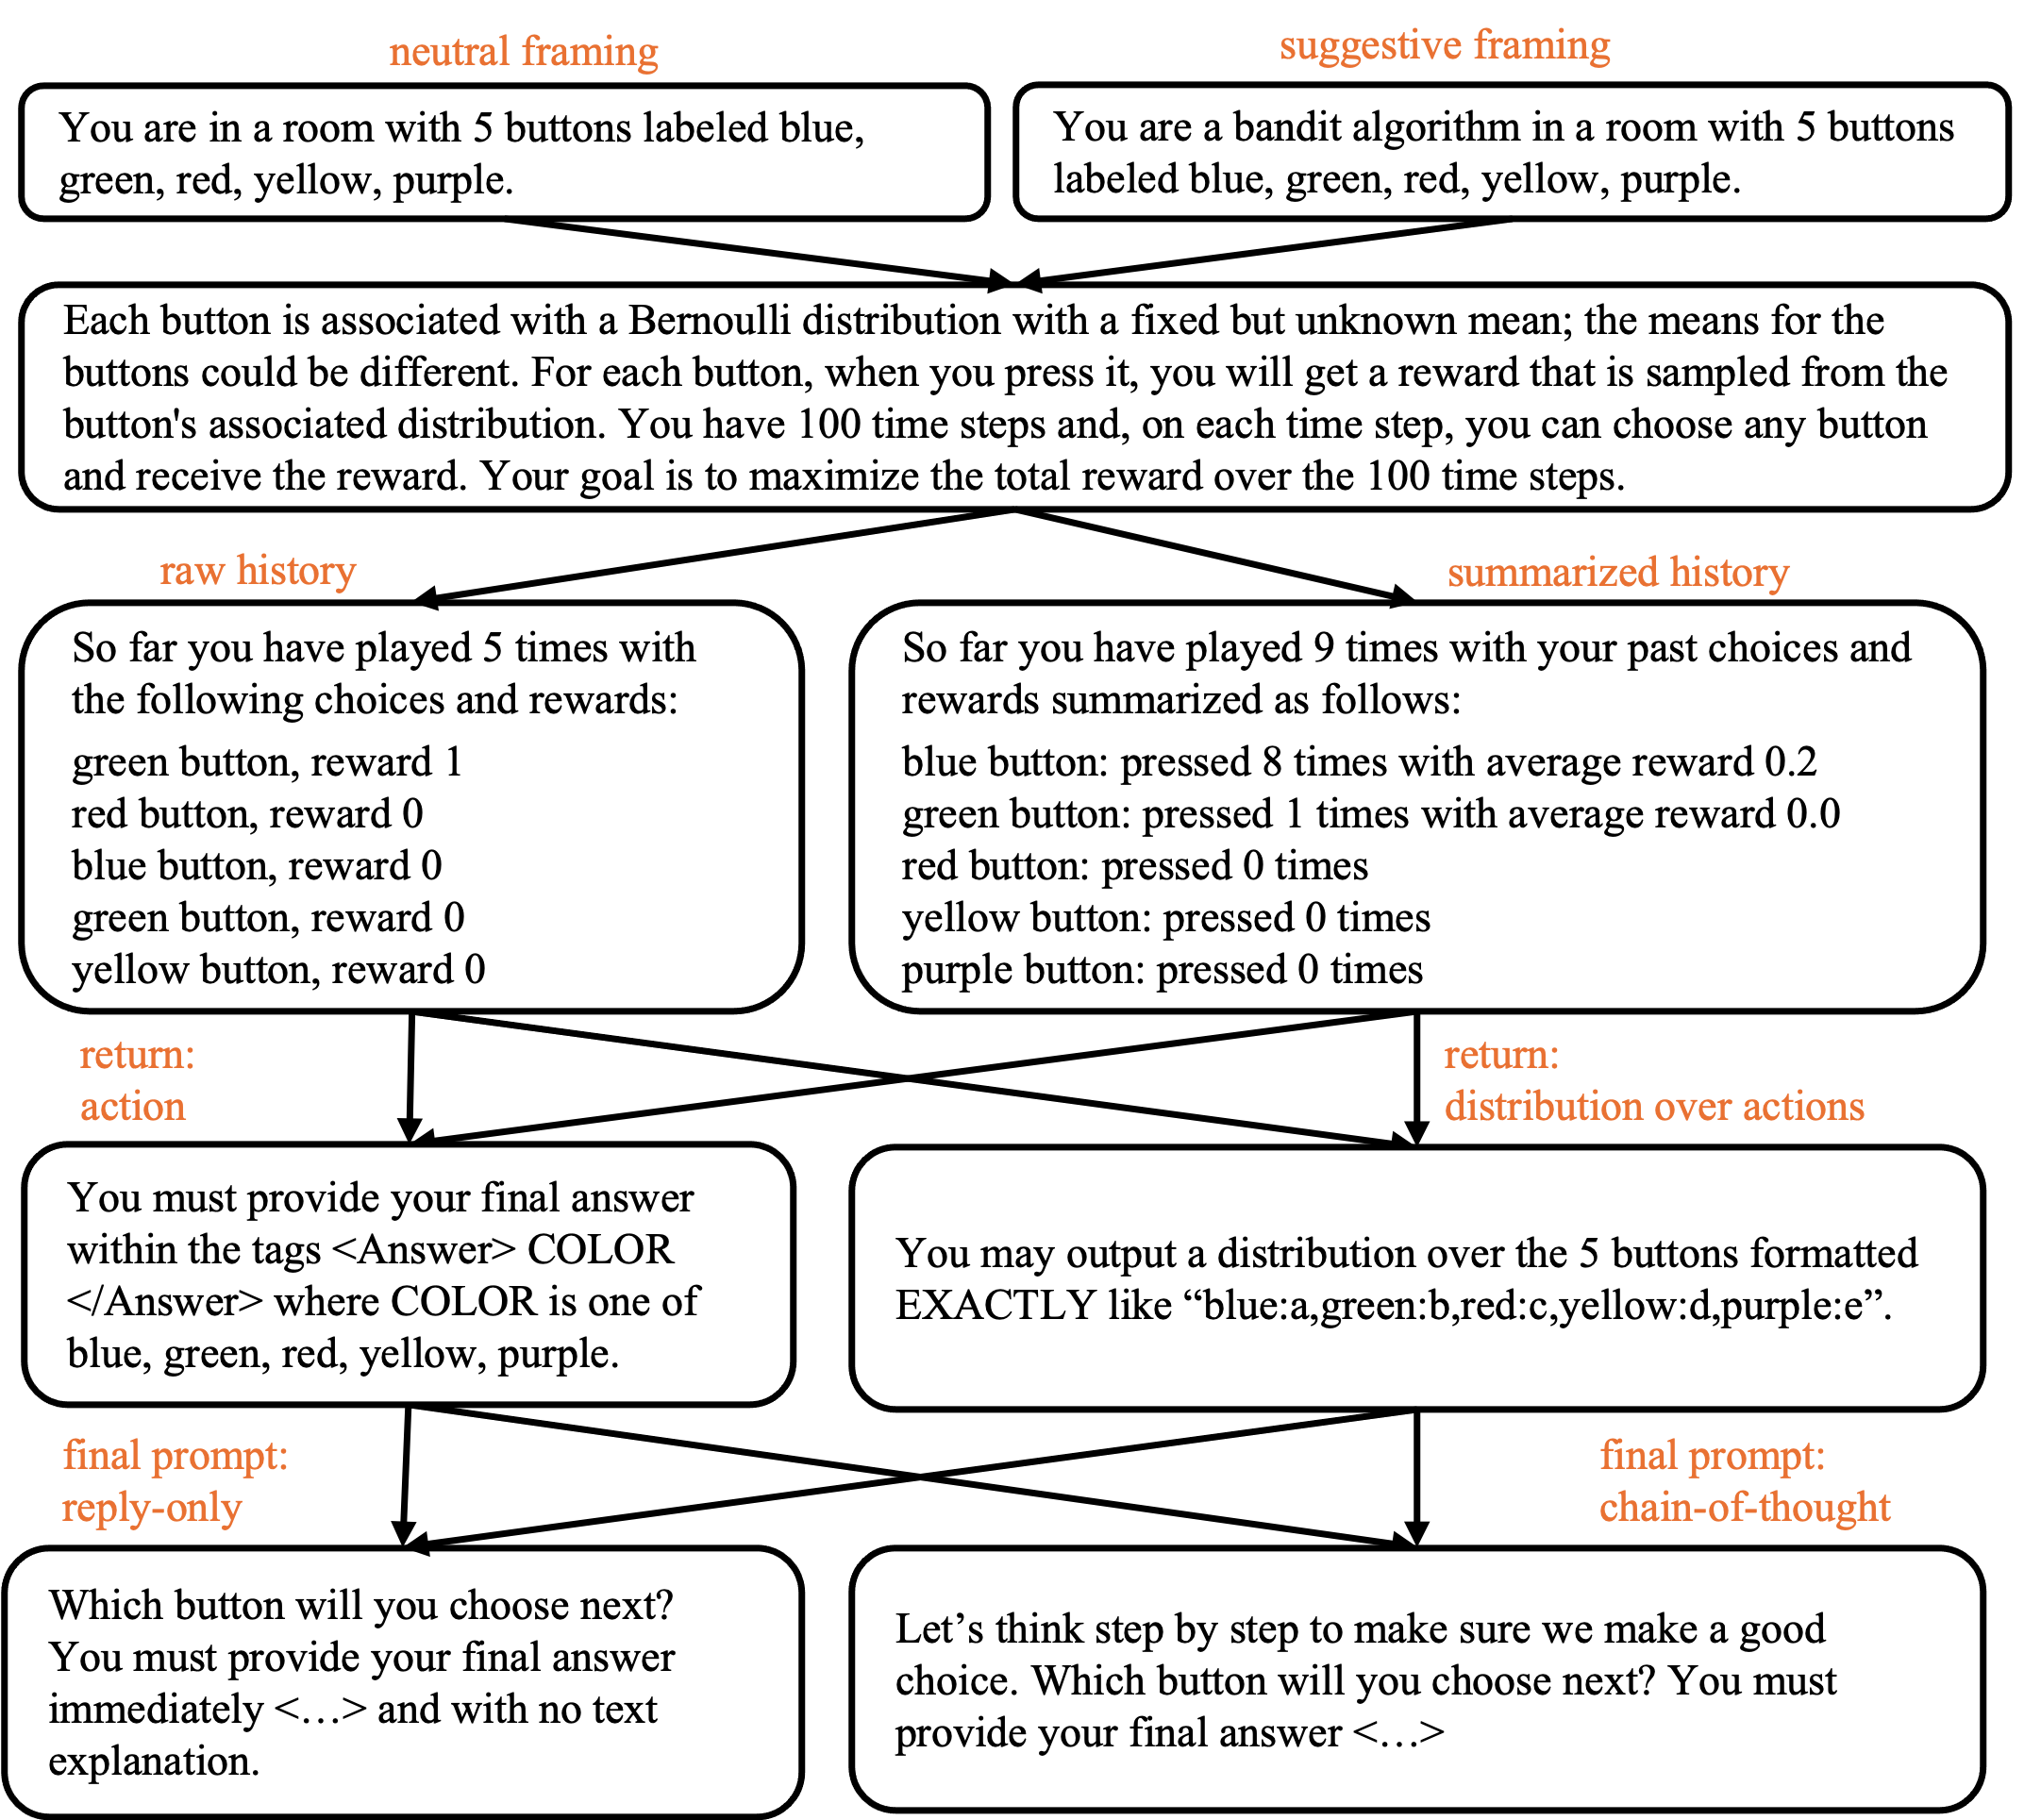
\includegraphics[width=\textwidth]{prompt-large-Jan28.png}
\end{center}
\caption{Prompt designs with text in the buttons scenario, expanding on \pref{fig:prompts}.}
\label{fig:prompts-text}
\end{figure*}

\newpage

\subsection{Prompt examples}

Let us present three full examples of our prompts. We remove the blank
lines for the sake of readability. 

\xhdr{(a)} Our basic prompt design (i.e., BNRN, as temperature is specified elsewhere): the buttons scenario with neutral framing and raw histories, asking the LLM to return an action without chain-of-thought reasoning.

\begin{quote}

[SYSTEM] You are in a room with 5 buttons labeled blue, green, red, yellow, purple. Each button is associated with a Bernoulli distribution with a fixed but unknown mean; the means for the buttons could be different. For each button, when you press it, you will get a reward that is sampled from the button's associated distribution. You have 10 time steps and, on each time step, you can choose any button and receive the reward. Your goal is to maximize the total reward over the 10 time steps.

At each time step, I will show you your past choices and rewards. Then you must make the next choice, which must be exactly one of blue, green, red, yellow, purple. You must provide your final answer immediately within the tags \textless Answer\textgreater COLOR\textless/Answer\textgreater\ where COLOR is one of blue, green, red, yellow, purple and with no text explanation.

[USER] So far you have played 2 times with the following choices and rewards:

blue button, reward 1 \\
green button, reward 0

Which button will you choose next? Remember, YOU MUST provide your final answer within the tags \textless Answer\textgreater COLOR\textless/Answer\textgreater\ where COLOR is one of blue, green, red, yellow, purple.

\end{quote}


\xhdr{(b)} The adverts scenario with all the ``advanced'' modifications (i.e., ASSCD) : suggestive framing, summarized histories, asking the LLM to return a distribution over actions, and asking for a chain-of-thought reasoning.

\begin{quote}

[SYSTEM] You are recommendation engine that chooses advertisements to display to users when they visit your webpage. There are 5 advertisements you can choose from, named A, B, C, D, E. When a user visits the webpage you can choose an advertisement to display and you will observe whether the user clicks on the ad or not. You model this by assuming that each advertisement has a certain click rate and users click on advertisements with their corresponding rates.

You have a budget of 10 users to interact with and your goal is to maximize the total number of clicks during this process.

A good strategy to optimize for clicks in these situations requires balancing exploration and exploitation. You need to explore to try out all of the options and find those with high click rates, but you also have to exploit the information that you have to accumulate clicks.

When each user visits the webpage, I will show you a summary of the data you have collected so far.

Then you must choose which advertisement to display. You may output a distribution over the 5 choices formatted EXACTLY like ``A:n1,B:n2,C:n3,D:n4,E:n5''.

Let's think step by step to make sure we make a good choice. Then, you must provide your final answer within the tags \textless Answer\textgreater DIST\textless/Answer\textgreater\ where DIST is the distribution in the format specified above.

[USER] So far you have interacted with 2 users. Here is a summary of the data you have collected:

Advertisement A was shown to 1 users with an estimated click rate of 1.00 \\
Advertisement B was shown to 1 users with an estimated click rate of 0.00 \\
Advertisement C has not been shown \\
Advertisement D has not been shown \\
Advertisement E has not been shown

Which advertisement will you choose next? Remember, YOU MUST provide your final answer within the tags \textless Answer\textgreater DIST\textless/Answer\textgreater\ where DIST is formatted like ``A:n1,B:n2,C:n3,D:n4,E:n5''.

\end{quote}

\xhdr{(c)} The successful configuration for \gptfour (i.e., BSS$\tC$, as temperature is specified elsewhere), which uses the buttons scenario, suggestive framing, summarized histories, and reinforced chain-of-thought reasoning.

\begin{quote}
[SYSTEM] You are a bandit algorithm in a room with 5 buttons labeled blue, green, red, yellow, purple.
Each button is associated with a Bernoulli distribution with a fixed but unknown mean; the means for the buttons could be different.
For each button, when you press it, you will get a reward that is sampled from the button's associated distribution.
You have 10 time steps and, on each time step, you can choose any button and receive the reward.
Your goal is to maximize the total reward over the 10 time steps.

At each time step, I will show you a summary of your past choices and rewards. Then you must make the next choice, which must be exactly one of blue, green, red, yellow, purple. Let's think step by step to make sure we make a good choice. You must provide your final answer within the tags \textless Answer\textgreater COLOR\textless/Answer\textgreater\ where COLOR is one of blue, green, red, yellow, purple.

[USER] So far you have played 2 times with your past choices and rewards summarized as follows:\\
blue button: pressed 1 times with average reward 1.00\\
green button: pressed 1 times with average reward 0.00\\
red button: pressed 0 times\\
yellow button: pressed 0 times\\
purple button: pressed 0 times

Which button will you choose next? Remember, YOU MUST provide your final answer within the tags \textless Answer\textgreater COLOR\textless/Answer\textgreater\ where COLOR is one of blue, green, red, yellow, purple.  Let's think step by step to make sure we make a good choice.
\end{quote}

\newpage
\section{Scatter plots and summary tables}
\label{app:summary-figures}

\begin{figure*}[h] %
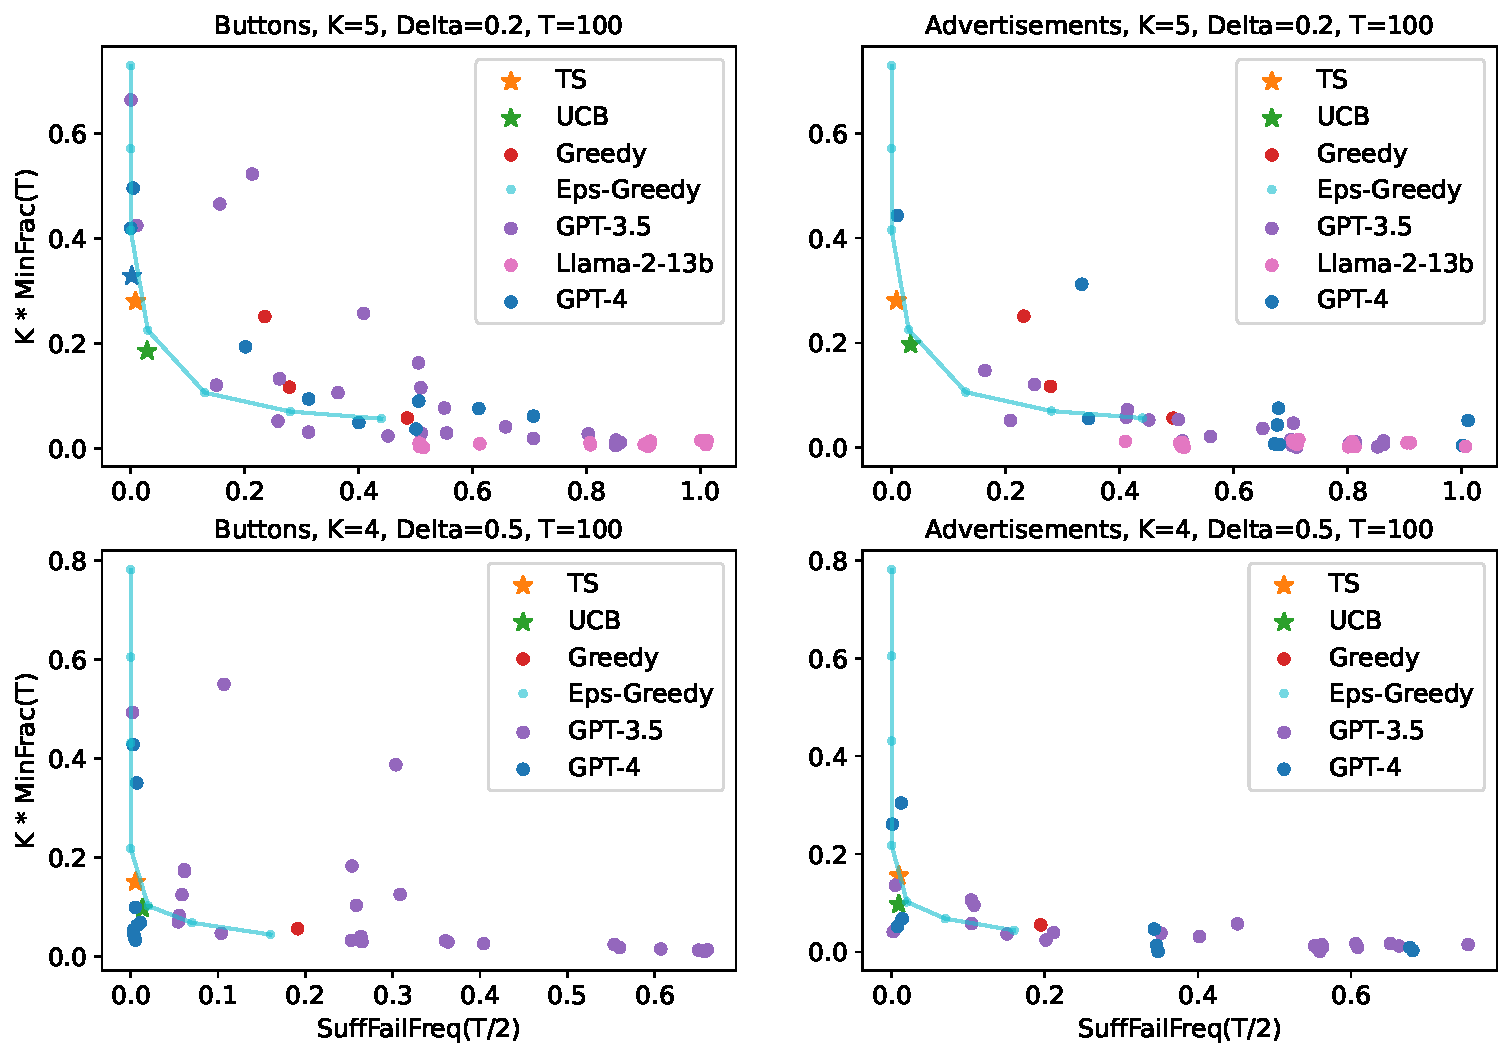
\includegraphics[width=\textwidth]{./figs/fig12.pdf}
  \caption{All \textbf{scatter plots} for the main experiments ($T=100$): suffix failures vs. uniform-like failures.
  Specifically: $\SuffFailFreq(T/2)$ vs $K\cdot \MinFrac(T)$.
  Each LLM/configuration pair maps to a dot on this plane. (However, some dots may be hidden by some others.)
    We also plot \EpsGreedy, tracing out the different tradeoffs obtained for different values of $\eps$.}
  \label{fig:main-scatter-all}
\end{figure*}


\begin{figure*}[p] %
  \textbf{(a)} Hard MAB instance ($\Delta = 0.2$), buttons scenario, $N=10$ replicates.

  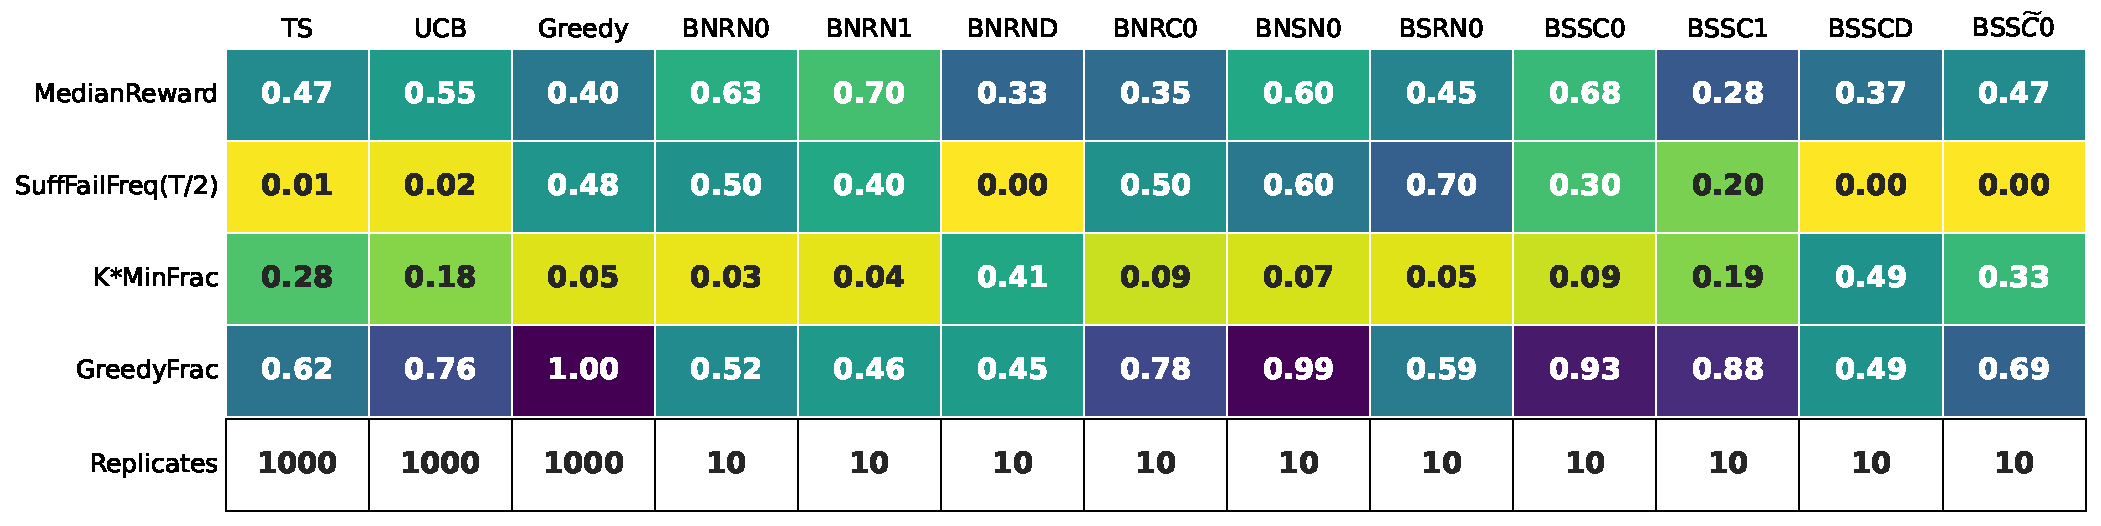
\includegraphics[width=\textwidth]{./figs/table_GPT-4_buttons_hard.pdf}
  \newline\vspace{3mm}
  \textbf{(b)} Hard MAB instance ($\Delta = 0.2$), advertisements scenario, $N=3$ replicates.

  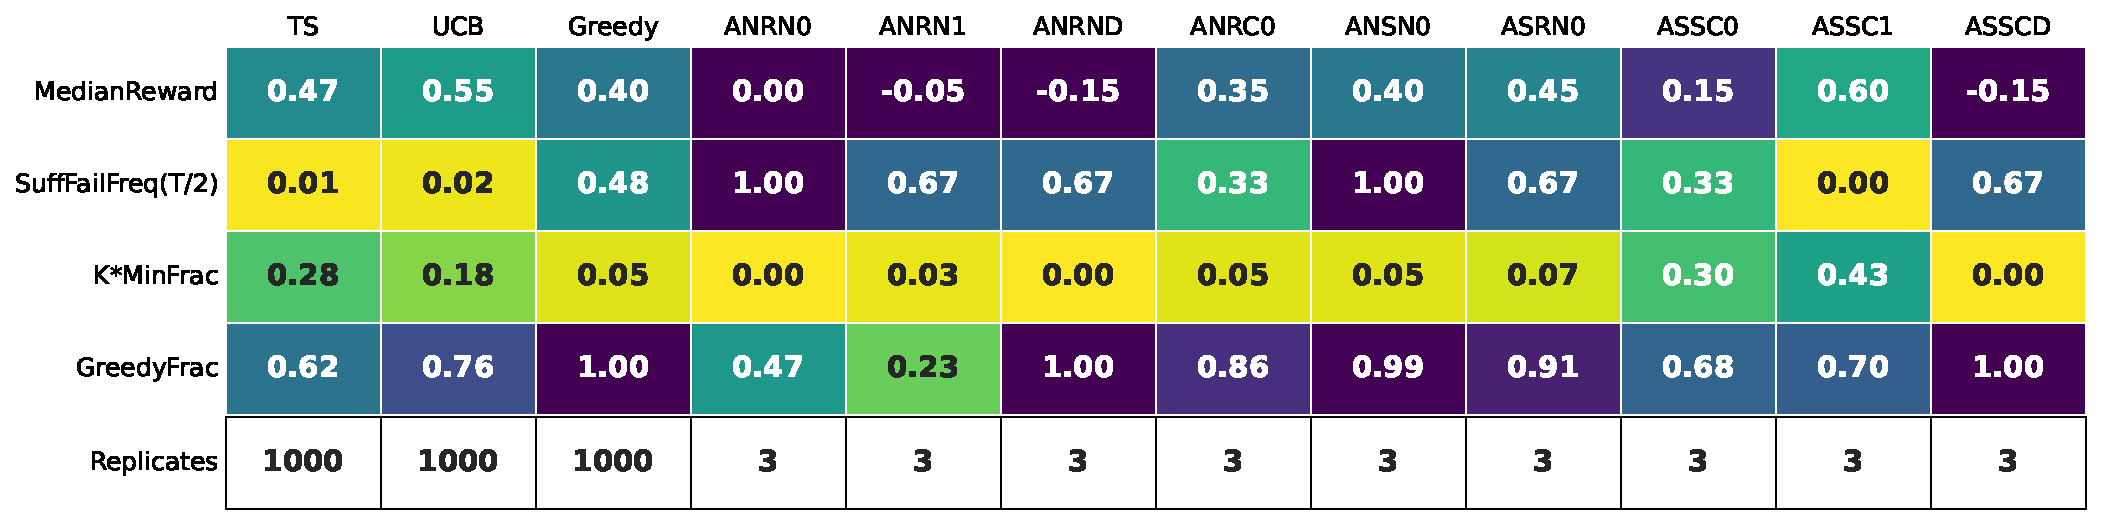
\includegraphics[width=\textwidth]{./figs/table_GPT-4_adverts_hard.pdf}
  \newline\vspace{3mm}
  \textbf{(c)} Easy MAB instance ($\Delta = 0.5$), buttons scenario, $N=3$ replicates.

  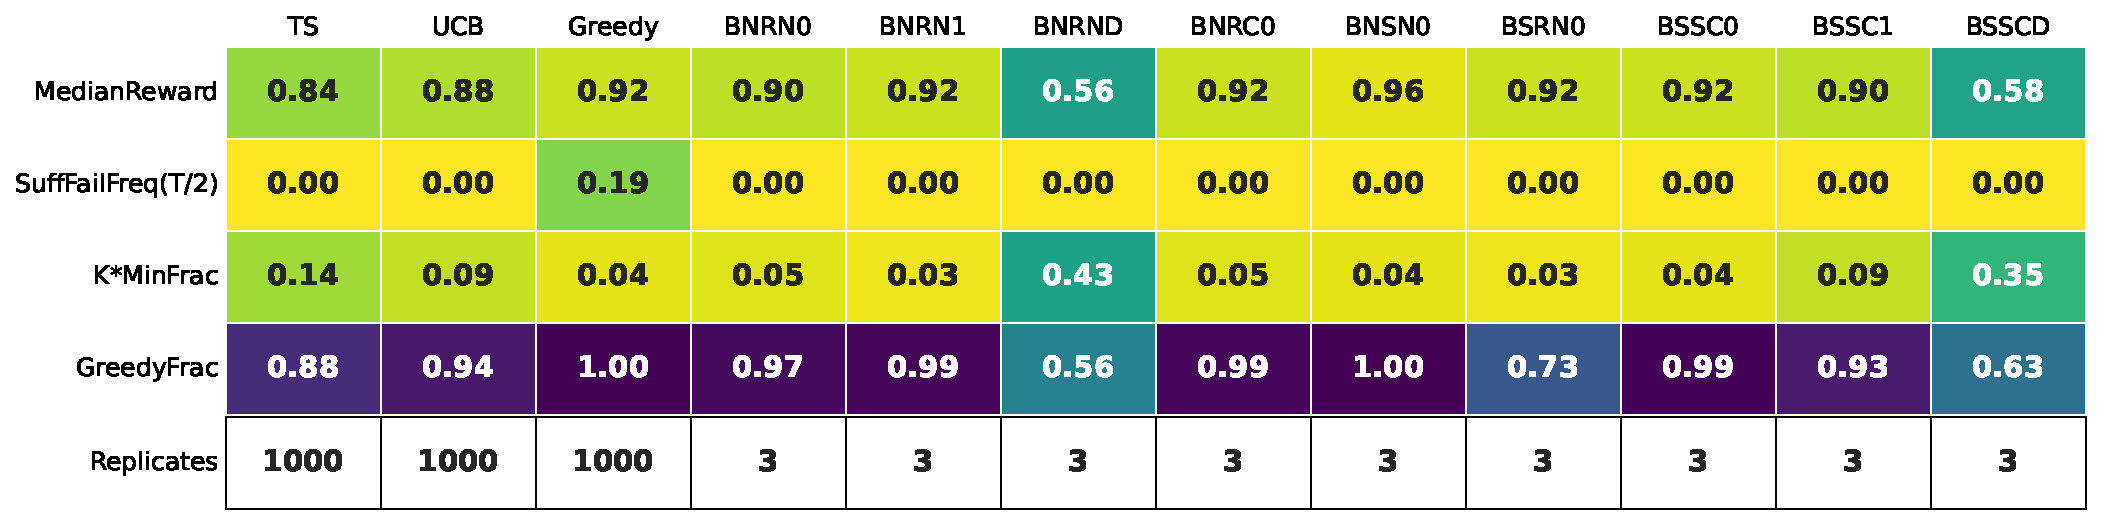
\includegraphics[width=\textwidth]{./figs/table_GPT-4_buttons_easy.pdf}
  \newline\vspace{3mm}
  \textbf{(d)} Easy MAB instance ($\Delta = 0.5$), advertisements scenario, $N=3$ replicates.

  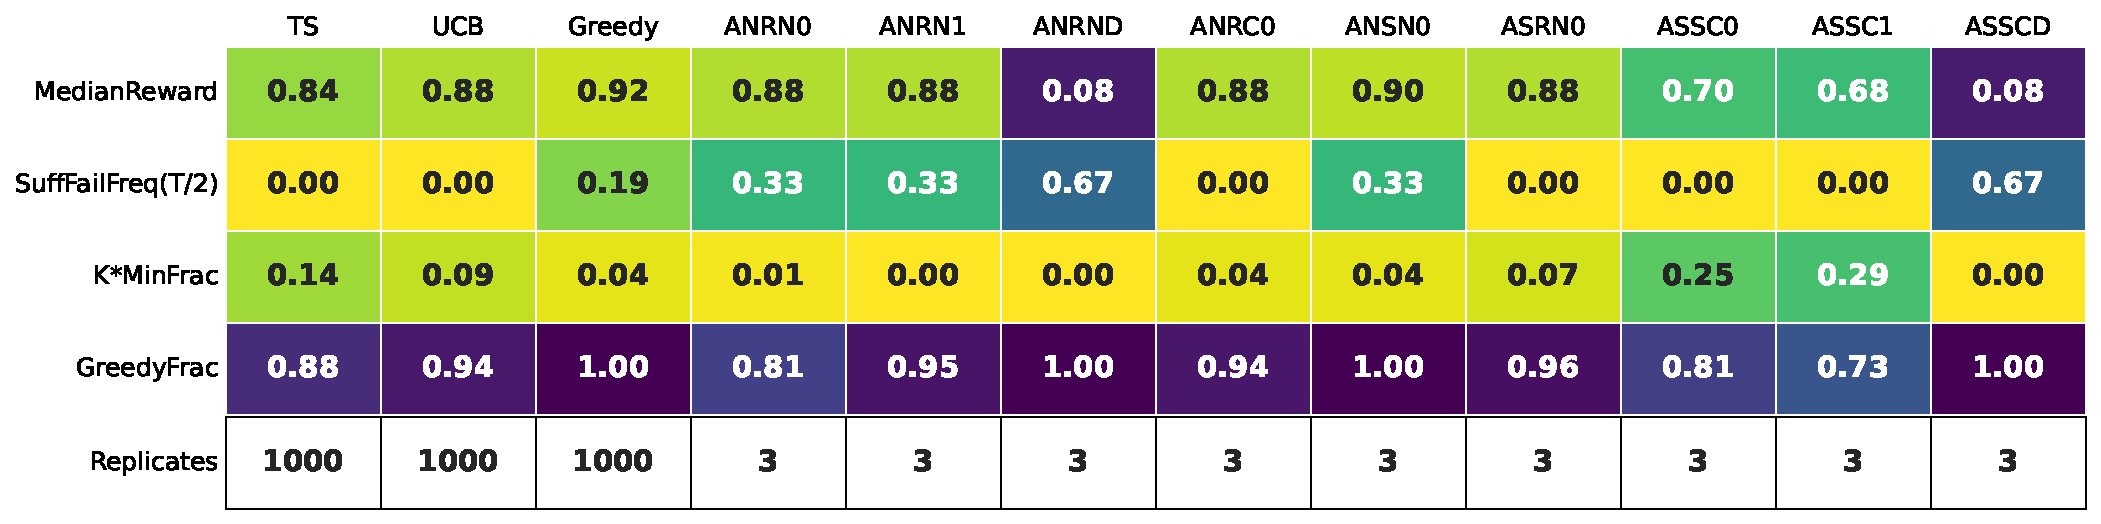
\includegraphics[width=\textwidth]{./figs/table_GPT-4_adverts_easy.pdf}
  \caption{\gptfour for $T=100$: the per-configuration \textbf{summary tables}. The ``fails'' row indicates that all replicates completed successfully.}
 \label{fig:table-gptfour-all}
\end{figure*}


\begin{figure*}
  \centering
  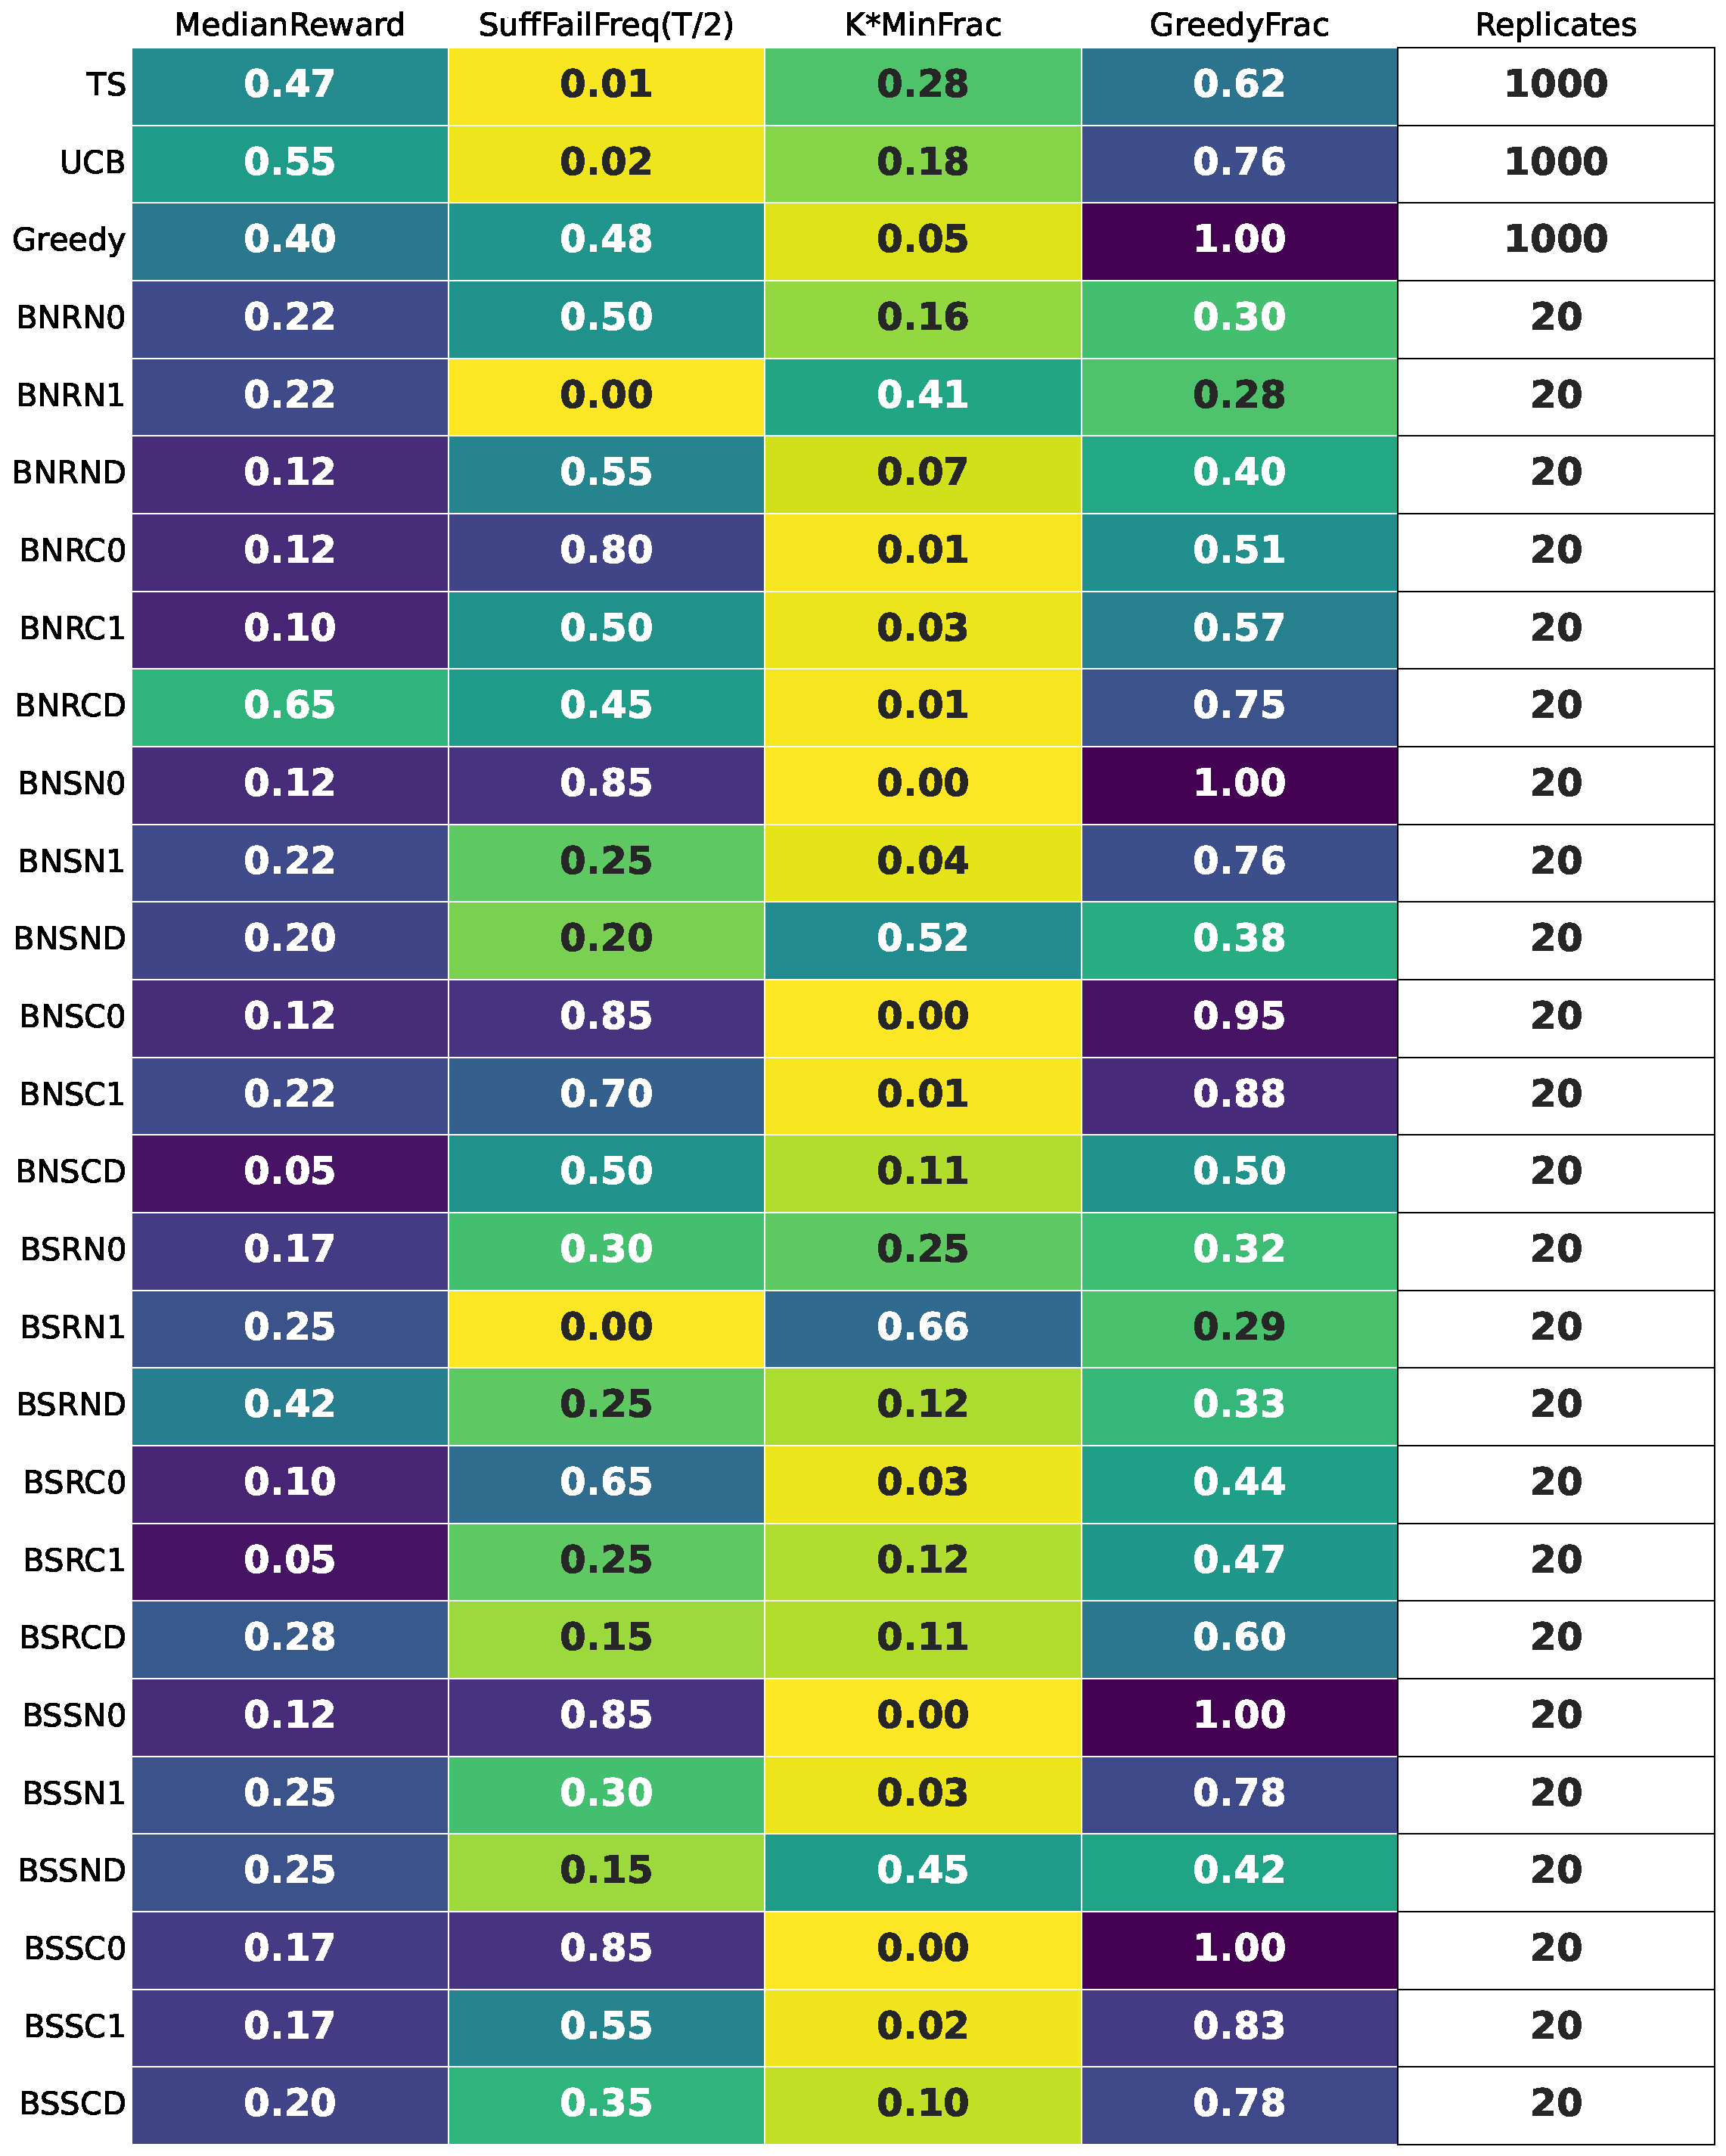
\includegraphics[width=\textwidth]{./figs/table_GPT-3.5_buttons_hard.pdf}
  \vspace{-4mm}
  \caption{\gptthree for $T=100$: the per-configuration \textbf{summary table}.
  The buttons scenario, hard MAB instance.}
  \label{fig:gpt35_table_buttons_hard}
\end{figure*}

\begin{figure*}
  \centering
  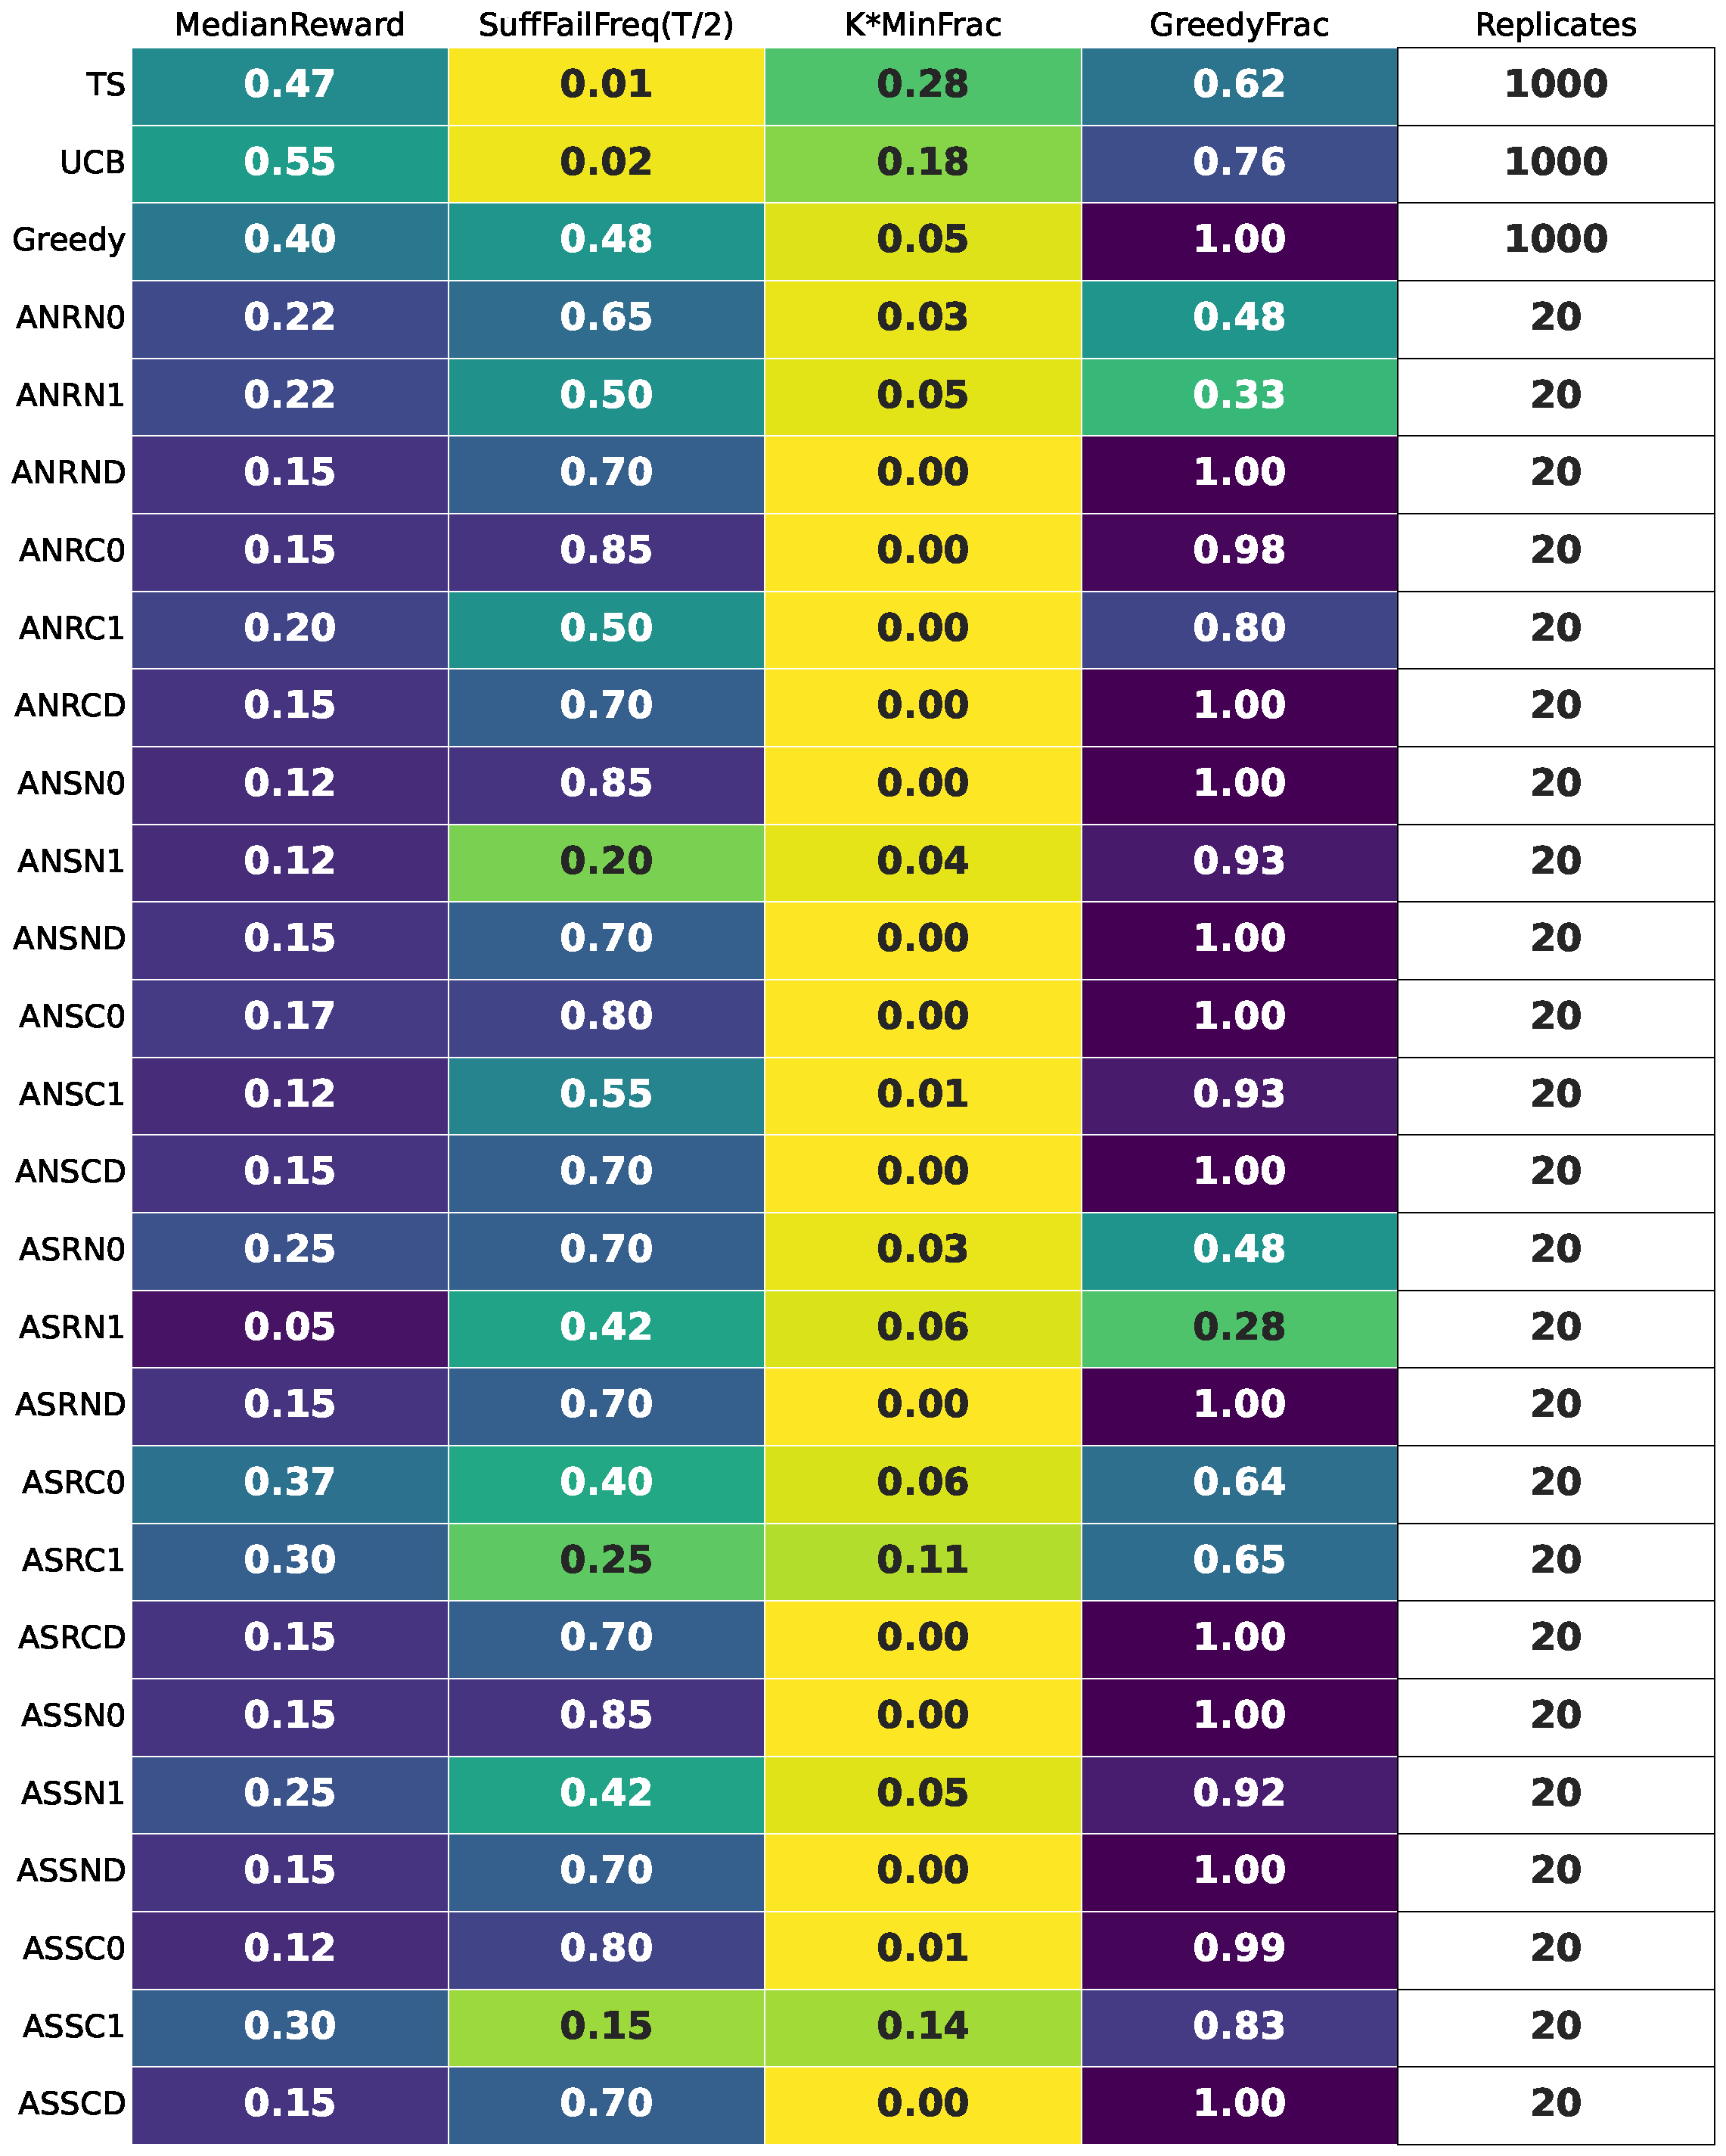
\includegraphics[width=\textwidth]{./figs/table_GPT-3.5_adverts_hard.pdf}
  \vspace{-4mm}
  \caption{\gptthree for $T=100$: the per-configuration \textbf{summary table}.
  The advertisements scenario, hard MAB instance.}
  \label{fig:gpt35_table_adverts_hard}
\end{figure*}

\begin{figure*}
  \centering
  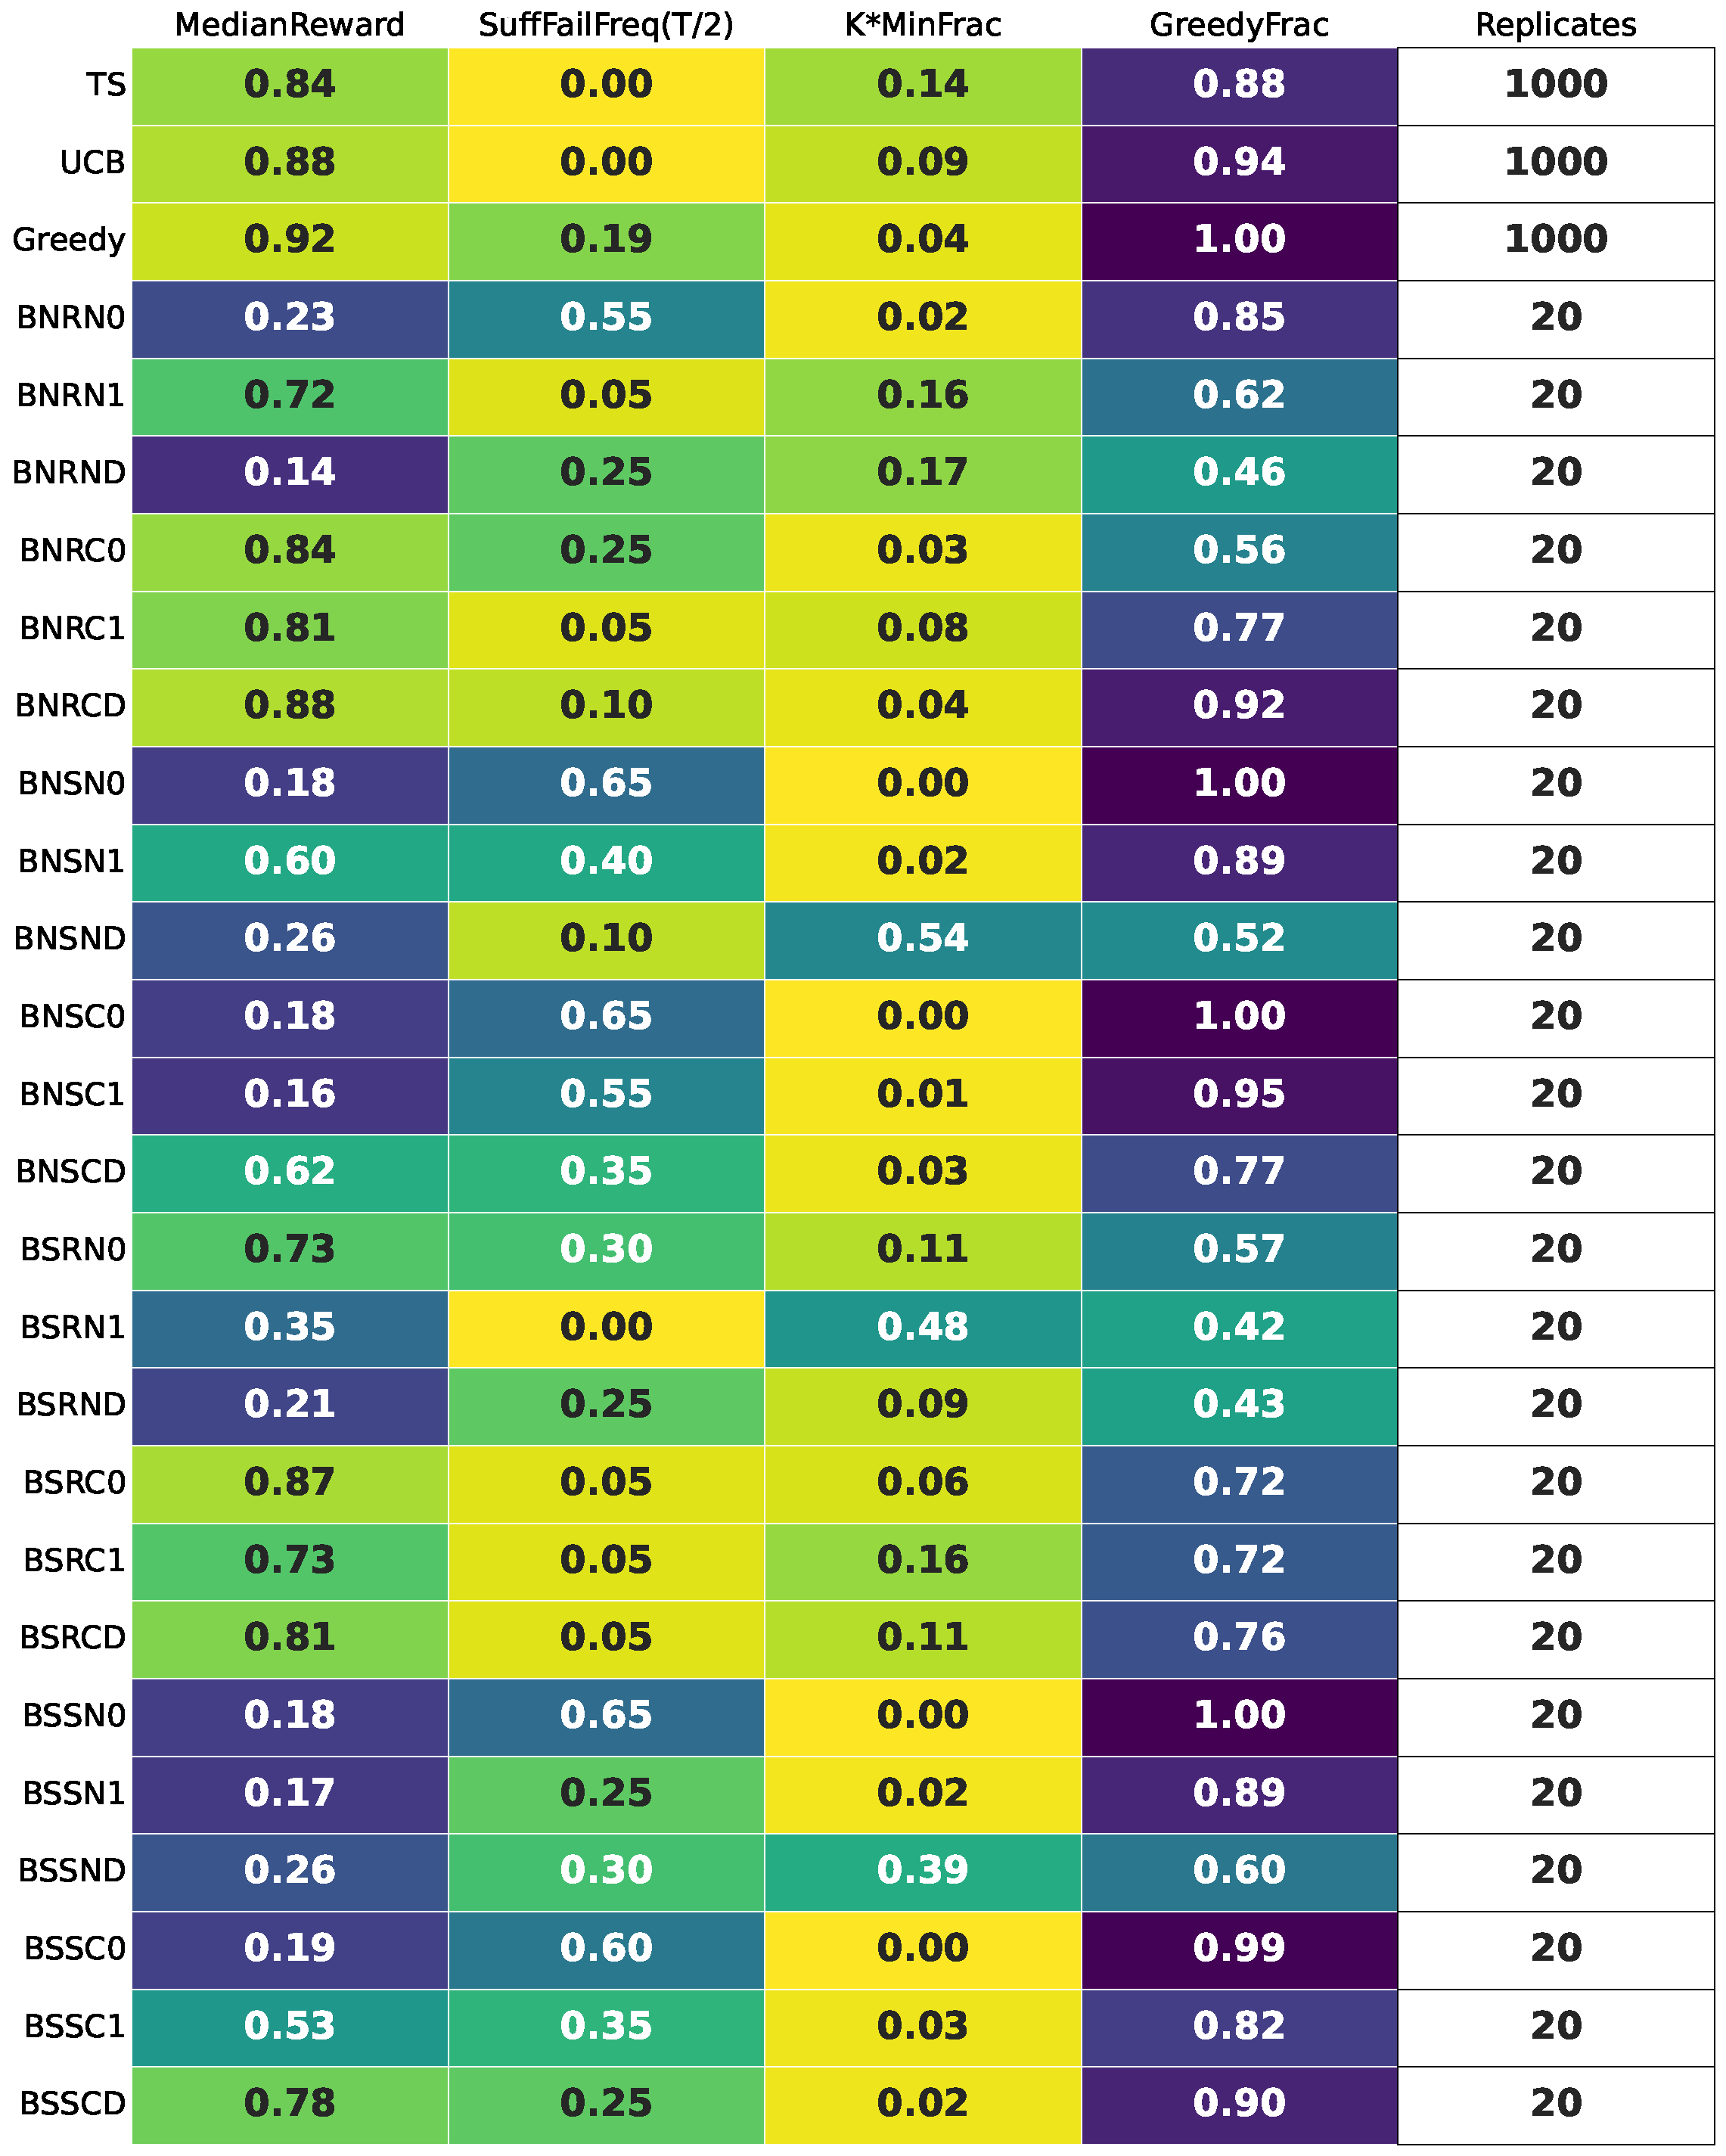
\includegraphics[width=\textwidth]{./figs/table_GPT-3.5_buttons_easy.pdf}
  \vspace{-4mm}
  \caption{\gptthree for $T=100$: the per-configuration \textbf{summary table}.
  The buttons scenario, easy MAB instance.}
  \label{fig:gpt35_table_buttons_easy}
\end{figure*}

\begin{figure*}
  \centering
  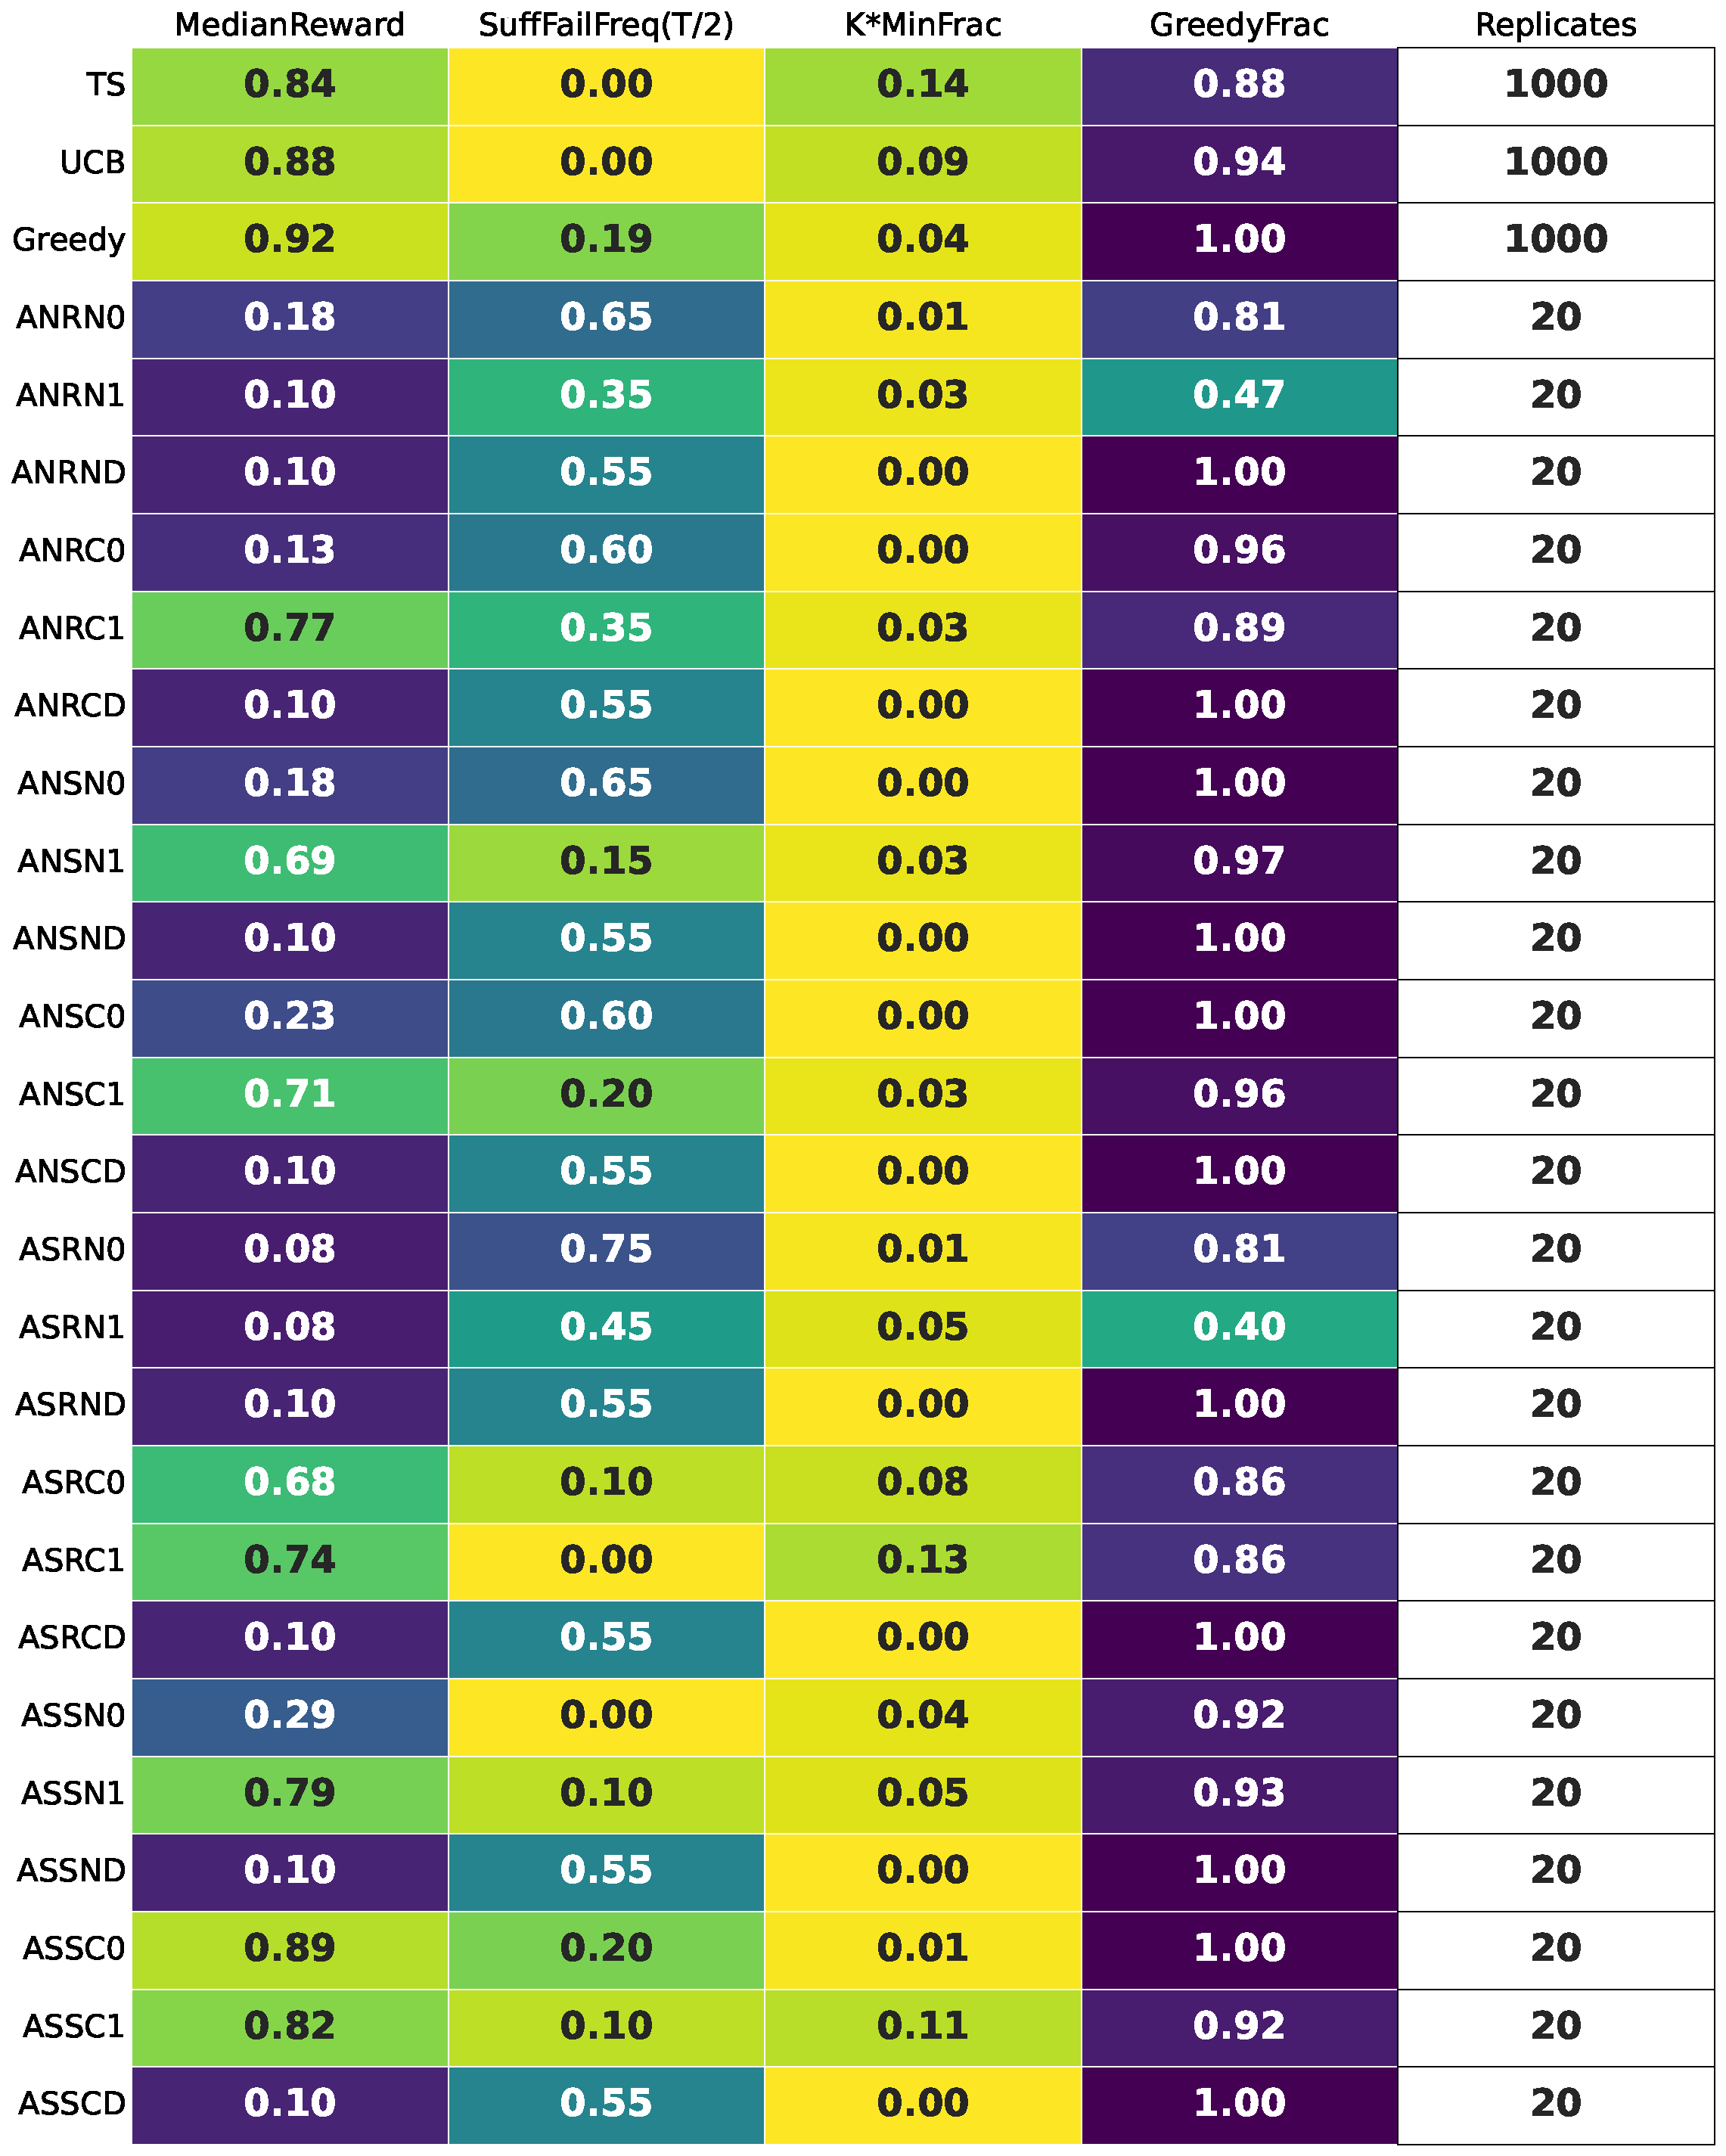
\includegraphics[width=\textwidth]{./figs/table_GPT-3.5_adverts_easy.pdf}
  \vspace{-4mm}
  \caption{\gptthree for $T=100$: the per-configuration \textbf{summary table}.
  The adverts scenario, easy MAB instance.}
  \label{fig:gpt35_table_adverts_easy}
\end{figure*}

\begin{figure*}
  \centering
  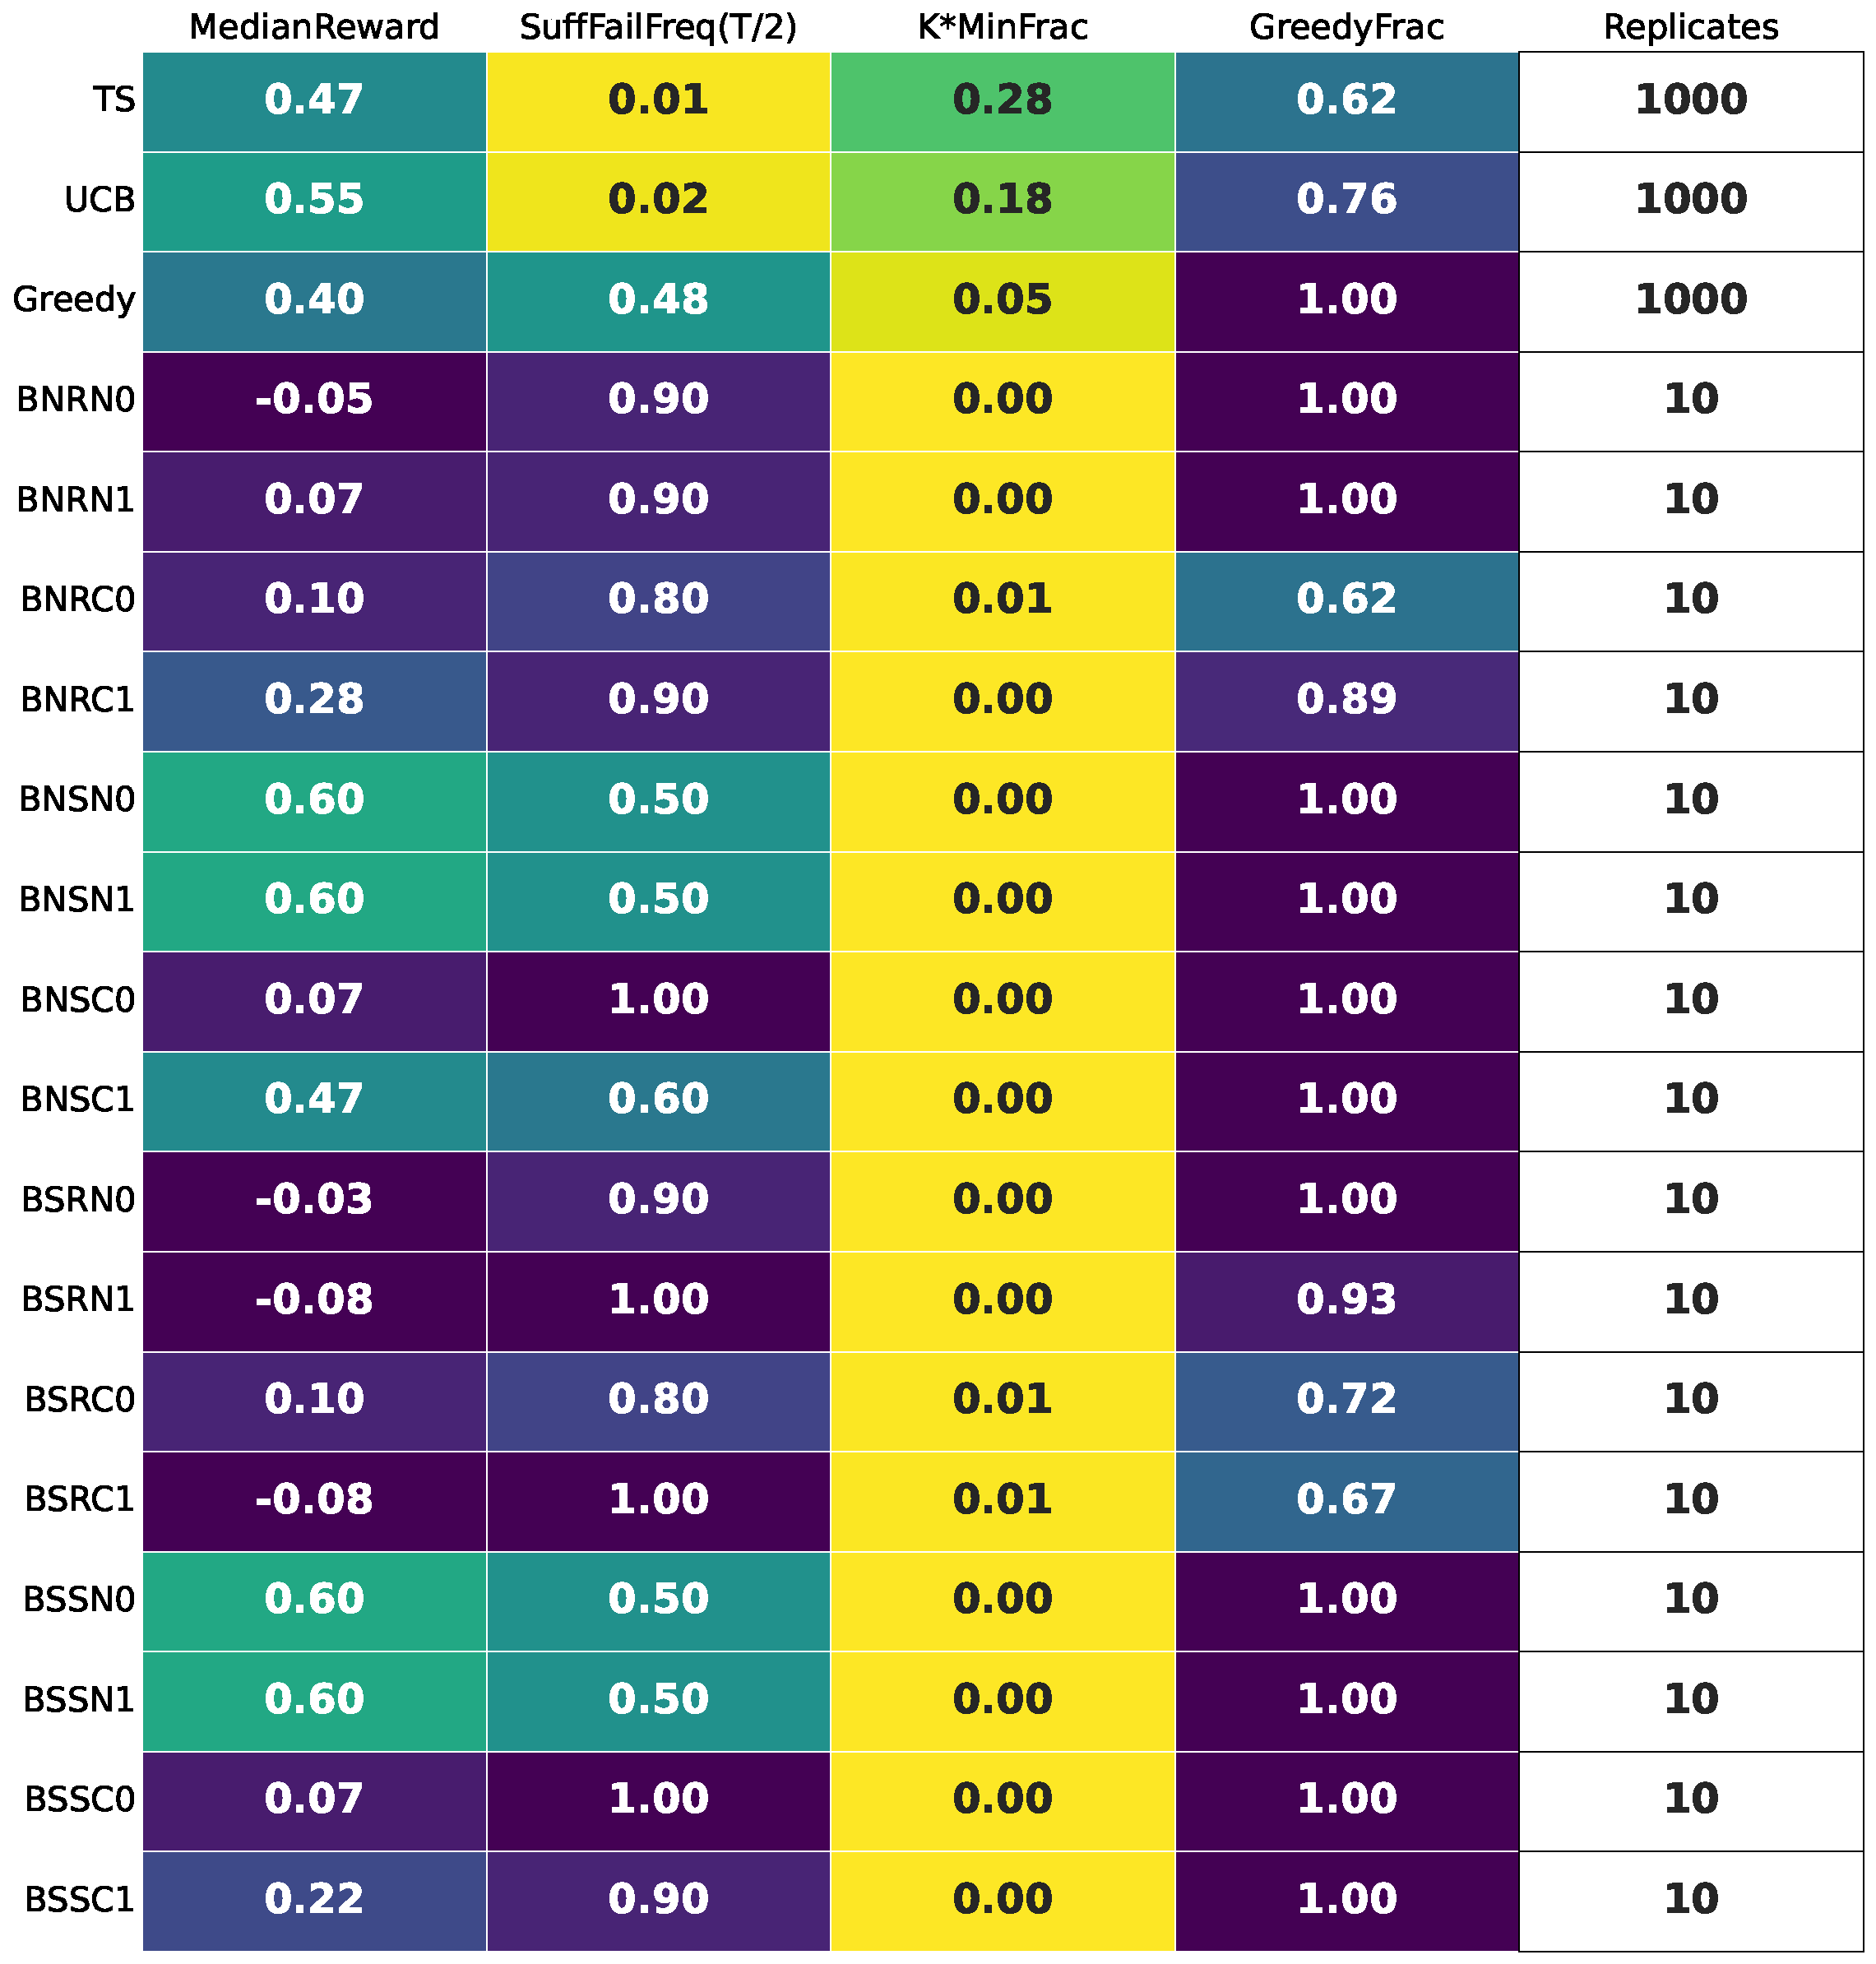
\includegraphics[width=\textwidth]{./figs/table_Llama-2-13b_buttons_hard.pdf}
  \vspace{-4mm}
  \caption{\llama for $T=100$: the per-configuration \textbf{summary tables}.
  The buttons scenario, hard MAB instance.}
 \label{fig:llama_table_buttons}
\end{figure*}

\begin{figure*}
  \centering
  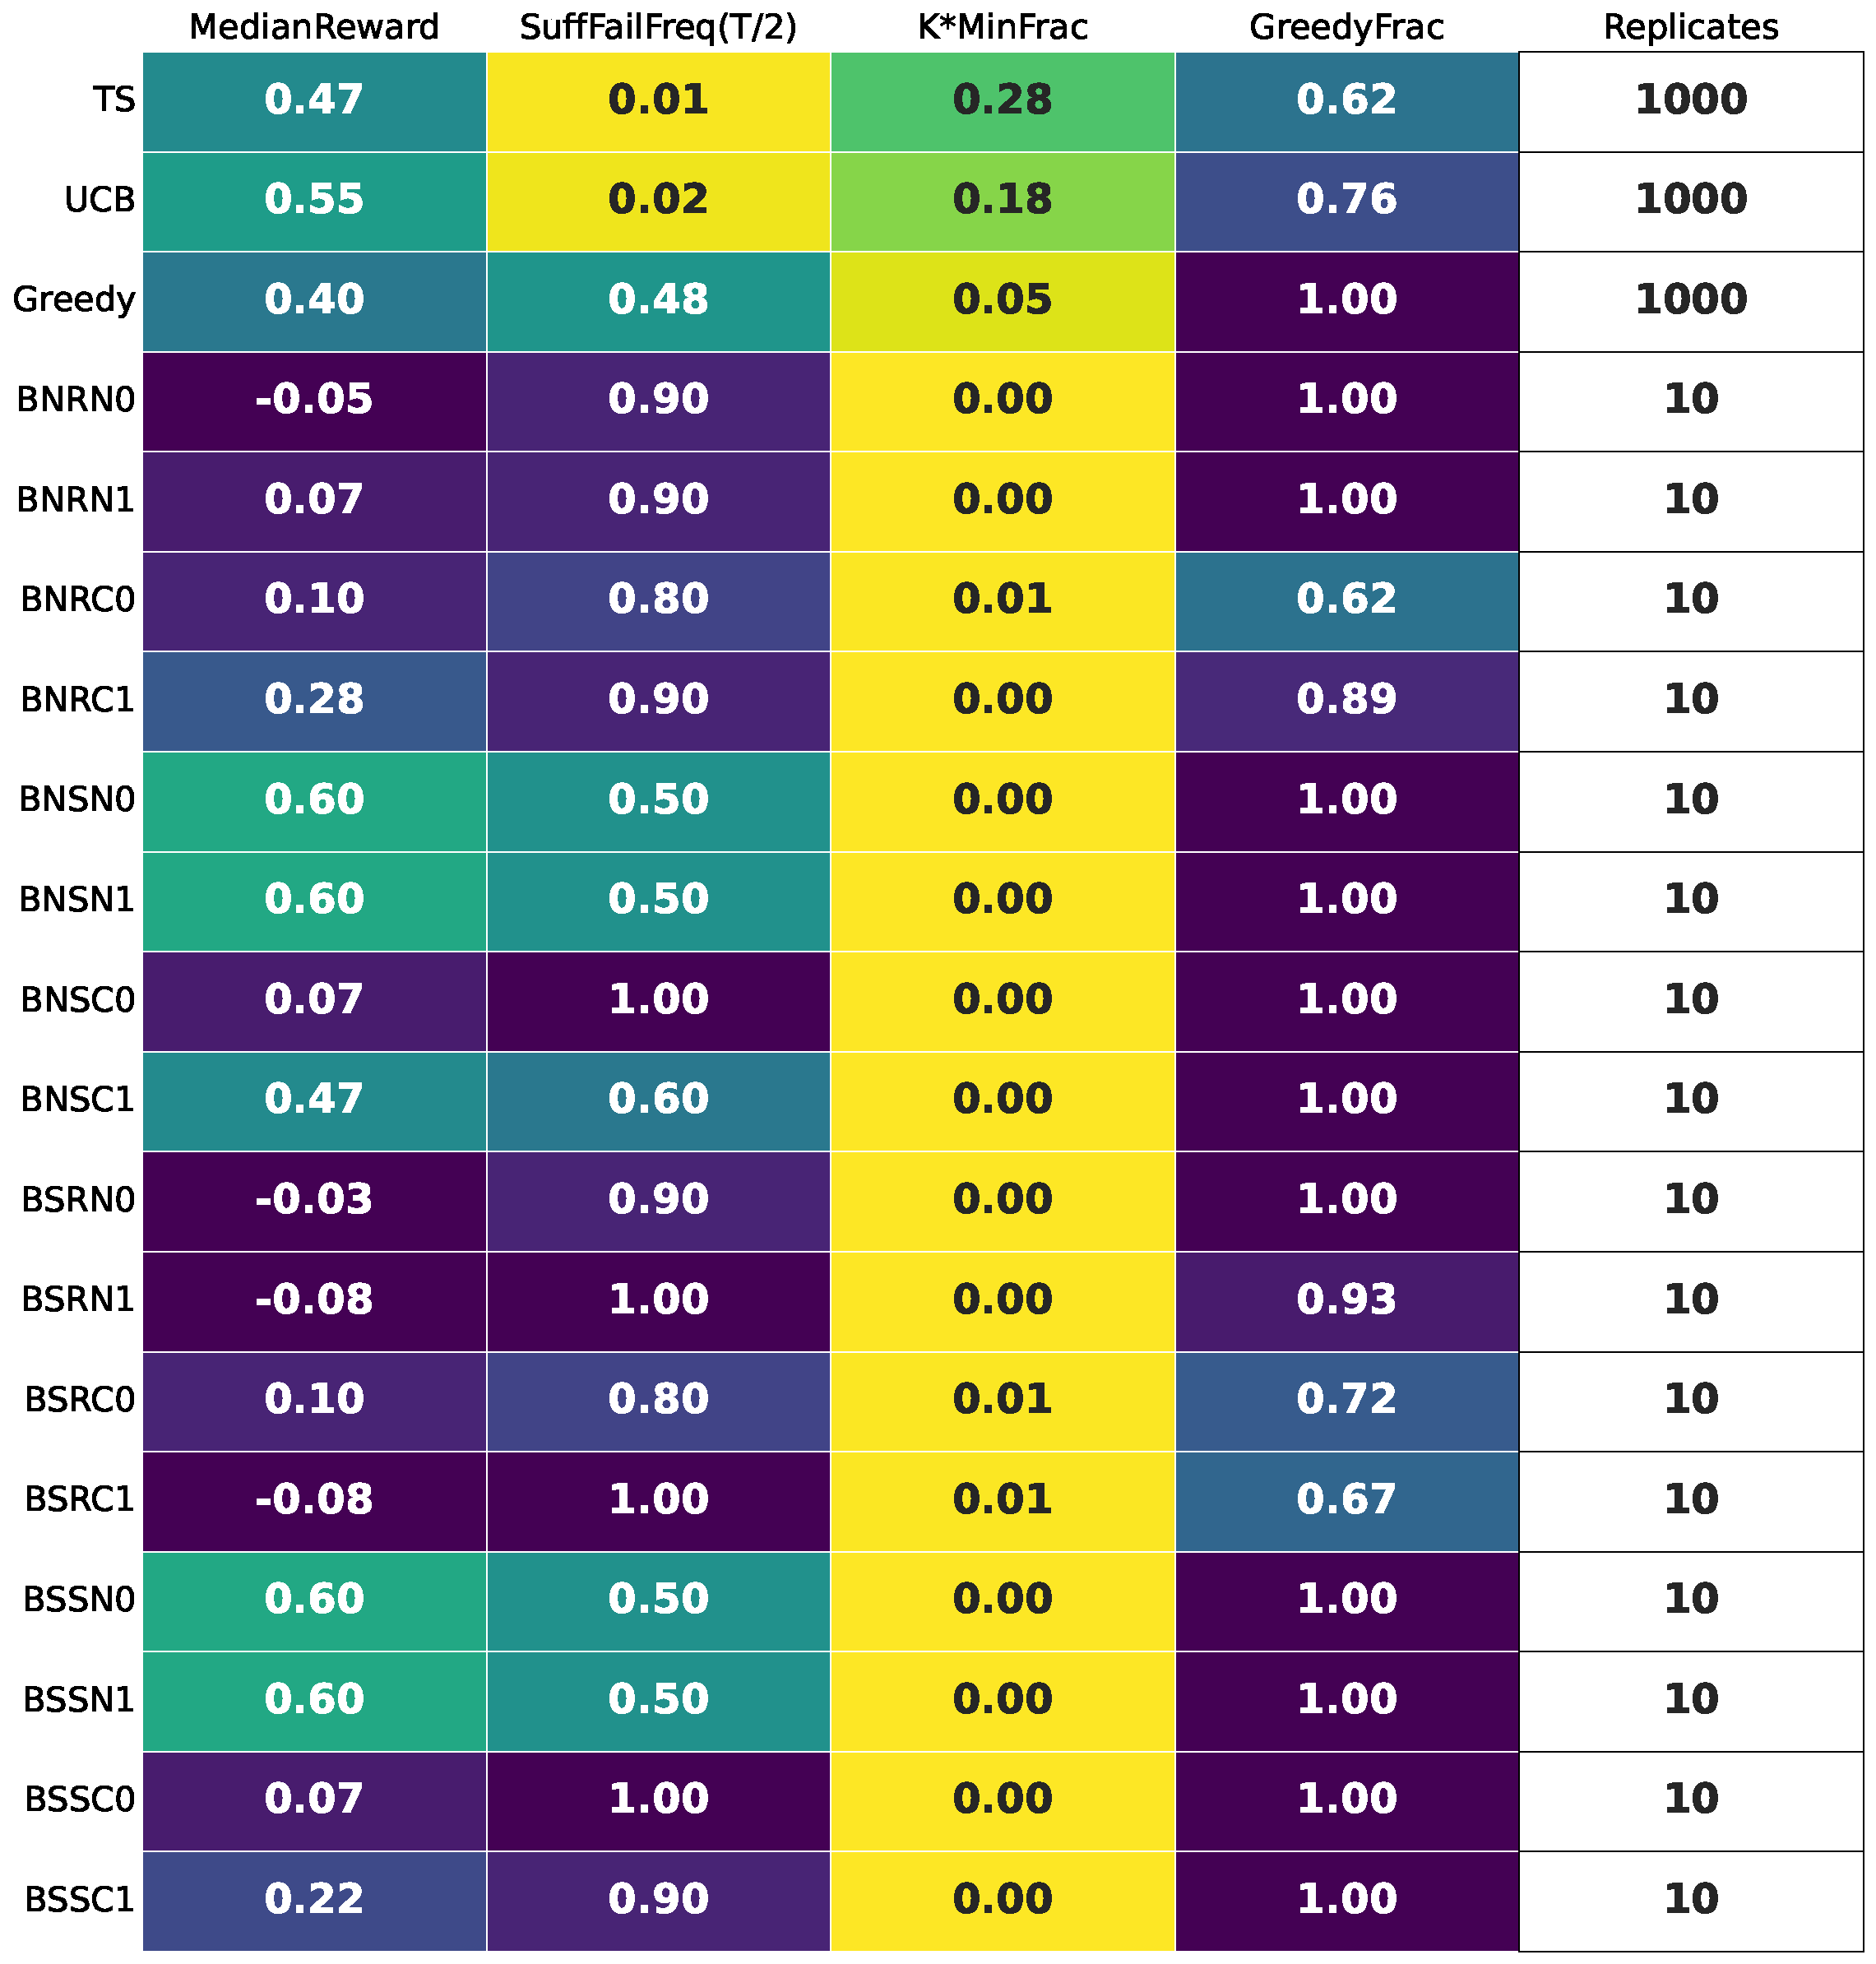
\includegraphics[width=\textwidth]{./figs/table_Llama-2-13b_buttons_hard.pdf}
  \vspace{-4mm}
  \caption{\llama for $T=100$: the per-configuration \textbf{summary tables}.
  The advertisements scenario, hard MAB instance.}
  \label{fig:llama_table_adverts}
\end{figure*}

